\documentclass[11pt,a4paper]{article}

\usepackage[margin=2.3cm]{geometry}
\usepackage{amsmath,amssymb,amsthm,bm}
\usepackage{graphicx}
\usepackage{booktabs}
\usepackage{xcolor}
\usepackage{tikz}
\usetikzlibrary{arrows.meta,positioning}
\usepackage{enumitem}
\usepackage{float}
\usepackage[colorlinks=true,linkcolor=blue!50!black,urlcolor=blue!50!black]{hyperref}

% ---------- helpers ----------
\newcommand{\E}{\mathbb{E}}
\newcommand{\N}{\mathcal{N}}
\newcommand{\x}{\mathbf{x}}
\newcommand{\abar}{\bar{\alpha}}
\newcommand{\todo}[1]{\textcolor{red}{\textbf{[TODO: #1]}}}
\newcommand{\answer}[1]{\par\noindent\textbf{Answer #1.}\ }
% include a figure if it exists, otherwise show a visible placeholder box
\newcommand{\safefig}[2]{%
  \IfFileExists{#1}{\includegraphics[width=#2]{#1}}%
  {\fbox{\parbox[c][3cm][c]{#2}{\centering\textcolor{red}{missing: \texttt{\detokenize{#1}}}}}}}

\title{\textbf{Assignment 2: Generative Models of Images}\\[2pt]
\large Generative AI \& LLM --- Fall 2026, ITU}
\author{Fahad Khalid}
\date{November 2026}

\begin{document}
\maketitle

\begin{center}
\begin{tabular}{@{}lp{0.68\linewidth}@{}}
\toprule
Code repository & \url{https://github.com/Fahad00888/genai-assignment2}\newline (private, shared with \texttt{HajraZawwar})\\
Model checkpoint & \todo{Google Drive link to \texttt{results/run\_10k/model.pt}}\\
Experiment tracking & \url{https://forge.coreweave.com/wandb/fahad00888-itu-lahore/DDPM_AFHQ}\\
\bottomrule
\end{tabular}
\end{center}

\tableofcontents
\newpage

%======================================================================
\section{Convolutional Neural Networks}
%======================================================================

\subsection*{1.1.a Padding}

With $m = h-\lfloor K_h/2\rfloor+(i-1)$ and $i\in\{1,\dots,K_h\}$, the extreme row indices are
\[
m_{\min} = 1-\Big\lfloor \tfrac{K_h}{2}\Big\rfloor \quad (h=1,\ i=1),
\qquad
m_{\max} = N_h + K_h - 1 - \Big\lfloor \tfrac{K_h}{2}\Big\rfloor \quad (h=N_h,\ i=K_h).
\]
Rows $m<1$ and $m>N_h$ are hallucinated, so the number of missing rows above is $1-m_{\min}$ and below is $m_{\max}-N_h = K_h-1-\lfloor K_h/2\rfloor = \lfloor (K_h-1)/2\rfloor$. Columns behave identically with $K_w$:
\[
\boxed{p_l=\Big\lfloor\frac{K_w}{2}\Big\rfloor,\qquad
p_r=\Big\lfloor\frac{K_w-1}{2}\Big\rfloor,\qquad
p_t=\Big\lfloor\frac{K_h}{2}\Big\rfloor,\qquad
p_b=\Big\lfloor\frac{K_h-1}{2}\Big\rfloor}
\]
Sanity checks: $K=3$ gives $1$ on both sides; an even kernel $K=4$ gives $2$ before and $1$ after; in all cases $p_t+p_b=K_h-1$ and $p_l+p_r=K_w-1$.

\subsection*{1.1.b Convolution on the explicitly padded input}

Define the padded tensor $\x'\in\mathbb{R}^{C\times(N_h+p_t+p_b)\times(N_w+p_l+p_r)}$ by
\[
x'_{c,a,b} =
\begin{cases}
x_{c,\,a-p_t,\,b-p_l} & \text{if } 1\le a-p_t\le N_h \text{ and } 1\le b-p_l\le N_w,\\
0 & \text{otherwise.}
\end{cases}
\]
The new layer is
\begin{align}
y'_{1,h,w} &= \theta_0 + \sum_{c=1}^{C}\sum_{i=1}^{K_h}\sum_{j=1}^{K_w}\theta_{c,i,j}\,x'_{c,m',n'}, \\
\text{where } m' &= h+(i-1) \text{ and } n' = w+(j-1), \\
&\forall h\in\{1,\dots,N_h\},\ w\in\{1,\dots,N_w\}.
\end{align}
\emph{Same output:} $m' = m+p_t$ and $n'=n+p_l$, so each product reads $x'_{c,m+p_t,n+p_l}=x_{c,m,n}$ for real pixels and $0$ exactly where the original formulation hallucinated a zero. \emph{Valid indices only:} $m'$ ranges over $1,\dots,N_h+K_h-1 = N_h+p_t+p_b$ and $n'$ over $1,\dots,N_w+p_l+p_r$, i.e.\ exactly the extent of $\x'$, and $\mathbf{y}'$ keeps the shape $1\times N_h\times N_w$.

\subsection*{1.1.c.i Role of skip connections in U-Net}

Skip connections take the encoder's feature map at each resolution and concatenate it to the decoder's feature map at the same resolution. Every downsampling step in the encoder discards spatial detail, so the bottleneck only carries a coarse, semantic summary (\emph{what} is in the image). Without skips the decoder would have to invent the exact boundaries from that summary and the masks would be blurry and misplaced. The skips hand back the high-resolution information (edges, precise positions) so the decoder can combine \emph{what} (from the deep path) with \emph{where} (from the skip), which is exactly what per-pixel segmentation needs. They also give gradients short paths to early layers, which eases training.

\subsection*{1.1.c.ii Spatial resolution through the network}

In the encoder each level \emph{halves} the height and width (2$\times$2 max-pooling in the original U-Net, a stride-2 convolution in our implementation) while the number of channels typically \emph{doubles}; the bottleneck has the smallest spatial size and the most channels. The decoder mirrors this: every level \emph{doubles} the height and width (up-convolution / upsampling) and halves the channels until the input resolution is restored. In our diffusion U-Net a $32\times32$ input goes $32\to16\to8\to4$ and back $4\to8\to16\to32$. (In the original paper the unpadded $3\times3$ convolutions also shave a border off each map, so a $572\times572$ input gives a $388\times388$ output.)

%======================================================================
\section{Encoder-only Transformers}
%======================================================================

\subsection*{2.1 Graphical model of a decoder-only Transformer}

A decoder-only Transformer factorises the joint with the chain rule, $p(w_1,\dots,w_N)=\prod_{n=1}^{N}p(w_n\mid w_1,\dots,w_{n-1})$, and makes \emph{no} conditional-independence assumption: through causal self-attention every word can depend on every earlier word. The directed graph therefore has an edge from \emph{every} earlier node to every later node (a fully connected DAG in left-to-right order). Drawn for $N=5$:

\begin{figure}[H]
\centering
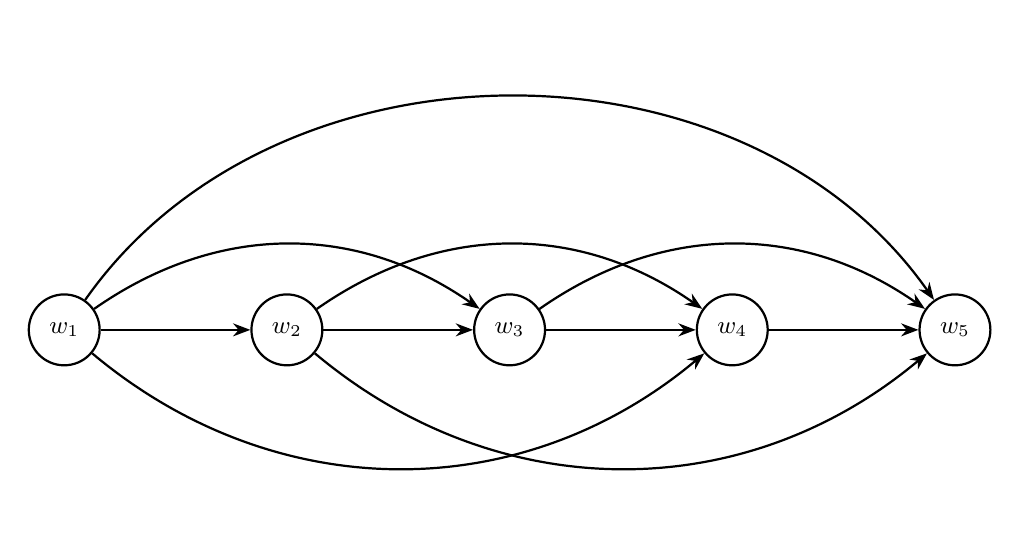
\begin{tikzpicture}[
  node distance=1.9cm,
  w/.style={circle,draw,thick,minimum size=9mm,font=\small},
  e/.style={-{Stealth[length=2.2mm]},thick}]
  \node[w] (w1) {$w_1$};
  \node[w,right=of w1] (w2) {$w_2$};
  \node[w,right=of w2] (w3) {$w_3$};
  \node[w,right=of w3] (w4) {$w_4$};
  \node[w,right=of w4] (w5) {$w_5$};
  % neighbours
  \draw[e] (w1)--(w2); \draw[e] (w2)--(w3); \draw[e] (w3)--(w4); \draw[e] (w4)--(w5);
  % skip-one
  \draw[e] (w1) to[bend left=35] (w3);
  \draw[e] (w2) to[bend left=35] (w4);
  \draw[e] (w3) to[bend left=35] (w5);
  % skip-two
  \draw[e] (w1) to[bend right=40] (w4);
  \draw[e] (w2) to[bend right=40] (w5);
  % skip-three
  \draw[e] (w1) to[bend left=55] (w5);
\end{tikzpicture}
\caption{Directed graphical model of $p(w_1,\dots,w_5)$ under a decoder-only Transformer: node $w_n$ has parents $w_1,\dots,w_{n-1}$. For general $N$ the same pattern continues (all $\binom{N}{2}$ forward edges).}
\end{figure}

\subsection*{2.2 Encoder-only vs.\ decoder-only sequence distributions}

\textbf{Encoder-only (with the given output layer).} Normalising the score vector gives a per-token distribution over tags, $p(y_n=v\mid w_{1:N}) = s_{n,v}/\sum_{v'} s_{n,v'}$ (a softmax of $\mathbf{W}\mathbf{h}_n+\mathbf{b}$). Because $\mathbf{h}_n$ comes from bidirectional attention, each tag sees the \emph{whole} sentence, but the tags are predicted independently of one another given the input:
\[
p(y_1,\dots,y_N\mid w_{1:N}) = \prod_{n=1}^{N} p(y_n\mid w_{1:N}).
\]
So this is a \emph{conditional} distribution over a label sequence of the \emph{same length} as the input, with no direct dependencies between output labels; it does not define a distribution over the words themselves and cannot generate text.

\textbf{Decoder-only.} It defines the full \emph{joint} distribution over the token sequence itself, $p(w_{1:N})=\prod_n p(w_n\mid w_{<n})$, with no independence assumptions, but each position only uses \emph{left} context. Because it is a proper generative model, it can sample sequences of arbitrary length token by token and can score any sequence.

\textbf{Best suited for.} Encoder-only: tasks where the input is fully given and we need a label per token or per sequence: POS tagging, named-entity recognition, sentence classification, extractive QA, retrieval embeddings. Decoder-only: tasks that require producing text: language modelling, completion, dialogue, summarisation or translation phrased as continuation, and scoring the likelihood of sequences.

%======================================================================
\section{Generative Adversarial Network (GAN)}
%======================================================================

Throughout, $\odot$ is element-wise multiplication and $m_{ij}=1$ marks a pixel to be filled in.

\subsection*{3.1.a Blank (a): composed output}
\[
\x' = \mathbf{m}\odot g_\theta(\x,\mathbf{m}) + (\mathbf{1}-\mathbf{m})\odot \x
\]
The model only decides the masked pixels; every intact pixel is copied from the input.

\subsection*{3.1.b Blank (b): masked squared error}
\[
\ell_{mse}(\theta) = \big\lVert \mathbf{m}\odot\big(g_\theta(\x,\mathbf{m})-\x\big)\big\rVert_2^2
= \sum_{i=1}^{N_h}\sum_{j=1}^{N_w} m_{ij}\,\big(g_\theta(\x,\mathbf{m})_{ij}-x_{ij}\big)^2
\]
Unmasked pixels are multiplied by $m_{ij}=0$ and do not contribute (equivalently $\ell_{mse}=\lVert\x'-\x\rVert_2^2$, since $\x'$ equals $\x$ outside the mask). Dividing by $\sum_{ij}m_{ij}$ gives a per-pixel mean if masks vary in size.

\subsection*{3.1.c Blank (c): GAN-style objective}
\[
\ell_{gan}(\phi,\theta) = \log d_\phi(\x) + \log\Big(1-d_\phi\big(\mathbf{m}\odot g_\theta(\x,\mathbf{m})+(\mathbf{1}-\mathbf{m})\odot\x\big)\Big),
\qquad \min_\theta\max_\phi\ \ell_{gan}(\phi,\theta).
\]
The discriminator ascends $\ell_{gan}$ (high probability for the real image, low for the inpainted one); the inpainting network descends it, which matches the update $\theta\leftarrow\theta-\eta\nabla_\theta\ell$ in the pseudo-code. Only the second term depends on $\theta$.

\subsection*{3.1.d Disadvantage of training with $\ell_{mse}$ only}

A masked region usually has many plausible fillings (different fur patterns, ear positions, \dots). Squared error is minimised by the \emph{average} of these possibilities, so an MSE-only model learns to output their mean: smooth, blurry patches without realistic texture, which stand out against the sharp surrounding pixels. The adversarial term instead penalises outputs that look unlike real images, pushing the model to commit to one sharp, realistic completion; combining both keeps the completion close to the truth (MSE) while staying on the manifold of natural images (GAN).

%======================================================================
\section{Variational Autoencoders}
%======================================================================

\subsection*{4.1 Which parameters receive gradients from $\widehat{\mathcal{R}}$?}

$\widehat{\mathcal{R}} = \log p_\theta(\x\mid z) = -\frac{(\x-w_3z-b_3)^2}{2\sigma^2} + \text{const}$.

\begin{enumerate}[label=(\alph*)]
\item \textbf{Black-box sampling:} only $\bm{w_3, b_3}$. The node ``$z\sim q_\phi(z\mid\x)$'' outputs a number with no differentiable path back to $\mu_\phi$ or $\sigma_\phi$, so $\partial\widehat{\mathcal{R}}/\partial w_1=\partial\widehat{\mathcal{R}}/\partial b_1=\partial\widehat{\mathcal{R}}/\partial w_2=\partial\widehat{\mathcal{R}}/\partial b_2=0$ in this graph, while $\widehat{\mathcal{R}}$ depends on $w_3,b_3$ directly.
\item \textbf{Reparameterisation:} \textbf{all six}, $\bm{w_1,b_1,w_2,b_2,w_3,b_3}$. Now $z=(w_1\x+b_1)+\exp\!\big(\tfrac{w_2\x+b_2}{2}\big)\,\epsilon$ is a deterministic, differentiable function of $\phi$ (randomness sits in $\epsilon$, which has no parameters), so the chain rule
$\frac{\partial\widehat{\mathcal{R}}}{\partial\phi}=\frac{\partial\widehat{\mathcal{R}}}{\partial z}\frac{\partial z}{\partial\phi}$ is non-zero for $w_1,b_1$ (through $\mu_\phi$) and $w_2,b_2$ (through $\sigma_\phi$), and $w_3,b_3$ still get gradients directly.
\end{enumerate}

\subsection*{4.2 Batch loss for video inputs}

Each video has $D = 3FHW$ pixels. Per-sample reconstruction error (MSE normalised by the number of pixels):
\[
\mathcal{L}^{rec}_i = \frac{1}{3FHW}\sum_{c=1}^{3}\sum_{f=1}^{F}\sum_{h=1}^{H}\sum_{w=1}^{W}\big(x_{i,cfhw}-\tilde{x}_{i,cfhw}\big)^2 .
\]
KL to the prior, using the hint with $\mu_0=\mu_\phi(x_i)$, $\sigma_0^2=\sigma^2_\phi(x_i)$, $\mu_1=0$, $\sigma_1^2=1$:
\[
D_{KL}\big(\N(\mu_\phi(x_i),\sigma_\phi^2(x_i))\,\|\,\N(0,1)\big)
=\frac12\Big(\log\frac{1}{\sigma_\phi^2(x_i)}+\sigma_\phi^2(x_i)+\mu_\phi(x_i)^2-1\Big).
\]
Summing per-sample losses, weighting the KL by $\beta$ and multiplying by $1/N$ (batch size $N$):
\[
\boxed{\;\mathcal{L}=\frac{1}{N}\sum_{i=1}^{N}\left[\frac{1}{3FHW}\big\lVert x_i-\tilde{x}_i\big\rVert_2^2
+\frac{\beta}{2}\Big(\sigma_\phi^2(x_i)+\mu_\phi(x_i)^2-1-\log\sigma_\phi^2(x_i)\Big)\right]\;}
\]
where $\lVert\cdot\rVert_2^2$ sums over all $3FHW$ entries.

\subsection*{4.3 Increasing $\beta$}

\textbf{The distribution $q_\phi(z\mid x)$ approaches $\N(0,I)$ but reconstructions become worse.}
A larger $\beta$ makes it more costly for the encoder to move $q_\phi(z\mid x)$ away from the prior, so the codes of different inputs overlap more and carry less information about $x$; the decoder then has less to work with and reconstructions degrade (the classic rate--distortion trade-off).

%======================================================================
\section{Understanding Diffusion Models}
%======================================================================

\subsection*{5.1 ELBO surgery}

\textbf{Step 1: expand both chains.} Substituting Eq.~(5) and Eq.~(6) into Eq.~(7) and taking logs,
\[
\log\frac{p_\theta(\x_{0:T})}{q(\x_{1:T}\mid\x_0)}
= \log p(\x_T) + \sum_{t=1}^{T}\log p_\theta(\x_{t-1}\mid\x_t) - \sum_{t=1}^{T}\log q(\x_t\mid\x_{t-1}).
\]

\textbf{Step 2: re-index the reverse terms} so that each one lines up with a forward term of the same $\x_t$. Peel off $t=1$ and shift $t\to t+1$ in the rest:
\[
\sum_{t=1}^{T}\log p_\theta(\x_{t-1}\mid\x_t)
=\log p_\theta(\x_0\mid\x_1) + \sum_{t=1}^{T-1}\log p_\theta(\x_t\mid\x_{t+1}).
\]
Split the last forward term off:
$\sum_{t=1}^{T}\log q(\x_t\mid\x_{t-1}) = \sum_{t=1}^{T-1}\log q(\x_t\mid\x_{t-1}) + \log q(\x_T\mid\x_{T-1}).$

\textbf{Step 3: regroup into $R + \sum \mathcal{L}_t + L_T$.}
\[
\log\frac{p_\theta(\x_{0:T})}{q(\x_{1:T}\mid\x_0)}
=\underbrace{\log p_\theta(\x_0\mid\x_1)}_{R}
-\sum_{t=1}^{T-1}\log\frac{q(\x_t\mid\x_{t-1})}{p_\theta(\x_t\mid\x_{t+1})}
+\underbrace{\log\frac{p(\x_T)}{q(\x_T\mid\x_{T-1})}}_{L_T}.
\]

\textbf{Step 4: take $\E_{q(\x_{1:T}\mid\x_0)}$ and marginalise.} Each term depends on only a few variables, so by $\E_{q(a,b,c)}[f(b,c)]=\E_{q(b,c)}[f(b,c)]$ the remaining variables integrate out of $q(\x_{1:T}\mid\x_0)$:
\begin{itemize}[nosep]
\item $R$ depends on $(\x_0,\x_1)$ only $\Rightarrow$ $\E_{q(\x_1\mid\x_0)}[\log p_\theta(\x_0\mid\x_1)]$;
\item the $t$-th summand depends on $(\x_{t-1},\x_t,\x_{t+1})$ only $\Rightarrow$ $\E_{q(\x_{t-1},\x_t,\x_{t+1}\mid\x_0)}[\,\cdot\,]$. (The Markov structure of the forward chain is what guarantees this triple marginal is all we need: given $\x_t$, everything before and after is irrelevant to the summand.)
\item $L_T$ depends on $(\x_{T-1},\x_T)$ only.
\end{itemize}

\textbf{Step 5: identify the constant.}
$\E[L_T] = -\E_{q(\x_{T-1}\mid\x_0)}\big[D_{KL}(q(\x_T\mid\x_{T-1})\,\|\,p(\x_T))\big]$ involves only the fixed prior $p(\x_T)=\N(\mathbf{0},\mathbf{I})$ and the fixed forward process (no learnable parameters), so it does not depend on $\theta$; call it $C$. Putting everything together:
\[
\log p(\x)\ \ge\ \E_{q(\x_1\mid\x_0)}\big[\log p_\theta(\x_0\mid\x_1)\big]
-\sum_{t=1}^{T-1}\underbrace{\E_{q(\x_{t-1},\x_t,\x_{t+1}\mid\x_0)}\!\left[\log\frac{q(\x_t\mid\x_{t-1})}{p_\theta(\x_t\mid\x_{t+1})}\right]}_{\mathcal{L}_t}
+C. \qquad\blacksquare
\]

\subsection*{5.2 Effect of $\mathcal{L}_t$ on the reverse process}

$\mathcal{L}_t$ enters the ELBO with a minus sign, so maximising the ELBO \emph{minimises} $\mathcal{L}_t$. Its numerator $q(\x_t\mid\x_{t-1})$ is fixed, so the only $\theta$-dependent part is $-\E_q[\log p_\theta(\x_t\mid\x_{t+1})]$: a cross-entropy that rewards the reverse step for placing high probability on the $\x_t$ values the forward process actually produced before it reached $\x_{t+1}$. In words, $\mathcal{L}_t$ forces each denoising step $p_\theta(\x_t\mid\x_{t+1})$ to \emph{undo one step of noising}, i.e.\ to be consistent with the forward chain at the same time step.
$\mathcal{L}_t$ grows without bound when $p_\theta$ puts almost no mass where the forward samples are; the ELBO term $-\mathcal{L}_t$ is maximised (and $\mathcal{L}_t$ minimised) when the reverse step matches the forward chain's own reverse conditional, $p_\theta(\x_t\mid\x_{t+1}) = q(\x_t\mid\x_{t+1},\x_0)$, at which point what remains of $\mathcal{L}_t$ no longer depends on $\theta$.

\subsection*{5.3 Sampling $\x_\tau$ with the one-step encoder}

Use Eq.~(9) as a recipe and walk the chain from $\x_0$:
\begin{enumerate}[nosep]
\item Start with the data point $\x_0$.
\item For $t=1,2,\dots,\tau$: draw $\bm{\epsilon}_t\sim\N(\mathbf{0},\mathbf{I})$ and set $\x_t=\sqrt{\alpha_t}\,\x_{t-1}+\sqrt{1-\alpha_t}\,\bm{\epsilon}_t$ (reparameterised sample of $\N(\sqrt{\alpha_t}\x_{t-1},(1-\alpha_t)\mathbf{I})$).
\item Return $\x_\tau$.
\end{enumerate}
Each iteration needs the previous one, so this costs $\tau$ Gaussian draws and updates: $\bm{O(\tau)}$ (times $O(d)$ per step for a $d$-pixel image).

\subsection*{5.4 Closed form of $q(\x_t\mid\x_0)$ (proof by induction)}

\emph{Claim:} $\x_t = \sqrt{\abar_t}\,\x_0 + \sqrt{1-\abar_t}\,\bm{\epsilon}$ with $\bm{\epsilon}\sim\N(\mathbf{0},\mathbf{I})$, i.e.\ $q(\x_t\mid\x_0)=\N(\sqrt{\abar_t}\x_0,(1-\abar_t)\mathbf{I})$.

\emph{Base case $t=1$:} By Eq.~(10) applied to Eq.~(9), $\x_1=\sqrt{\alpha_1}\x_0+\sqrt{1-\alpha_1}\bm{\epsilon}_1$, and $\abar_1=\alpha_1$. \checkmark

\emph{Inductive step:} assume $\x_{t-1}=\sqrt{\abar_{t-1}}\x_0+\sqrt{1-\abar_{t-1}}\,\bm{\epsilon}'$. One more forward step with fresh, independent noise $\bm{\epsilon}_t$:
\begin{align*}
\x_t &= \sqrt{\alpha_t}\,\x_{t-1}+\sqrt{1-\alpha_t}\,\bm{\epsilon}_t\\
&= \sqrt{\alpha_t\abar_{t-1}}\,\x_0 + \underbrace{\sqrt{\alpha_t(1-\abar_{t-1})}\,\bm{\epsilon}' + \sqrt{1-\alpha_t}\,\bm{\epsilon}_t}_{\text{sum of two independent zero-mean Gaussians}}.
\end{align*}
The sum of independent Gaussians is Gaussian with the variances added:
$\alpha_t(1-\abar_{t-1})+(1-\alpha_t)=1-\alpha_t\abar_{t-1}=1-\abar_t$, using $\abar_t=\alpha_t\abar_{t-1}$. Hence the noise part equals $\sqrt{1-\abar_t}\,\bm{\epsilon}$ in distribution, with $\bm{\epsilon}\sim\N(\mathbf{0},\mathbf{I})$, and
\[
\x_t=\sqrt{\abar_t}\,\x_0+\sqrt{1-\abar_t}\,\bm{\epsilon}
\quad\Longleftrightarrow\quad
q(\x_t\mid\x_0)=\N\big(\x_t;\sqrt{\abar_t}\,\x_0,(1-\abar_t)\mathbf{I}\big). \qquad\blacksquare
\]

\subsection*{5.5 Sampling $\x_\tau$ in closed form}

\begin{enumerate}[nosep]
\item Precompute $\abar_t=\prod_{i\le t}\alpha_i$ for all $t$ once (a cumulative product, done once before training; our code stores it as a buffer).
\item Draw a single $\bm{\epsilon}\sim\N(\mathbf{0},\mathbf{I})$.
\item Return $\x_\tau=\sqrt{\abar_\tau}\,\x_0+\sqrt{1-\abar_\tau}\,\bm{\epsilon}$.
\end{enumerate}
With $\abar$ precomputed this is a table lookup plus one noise draw: $\bm{O(1)}$ in $\tau$ (vs.\ $O(\tau)$ in 5.3). Even computing $\abar_\tau$ on the fly costs only $\tau$ scalar multiplications and still a single image-sized noise draw. This is what lets training pick a random $t$ per image in constant time.

%======================================================================
\section{Programming: Diffusion Models}
%======================================================================

\subsection*{Setup and implementation notes}

\begin{itemize}[nosep]
\item \textbf{Data and model.} AFHQ cat training split (5{,}153 images, resized to 35 and randomly cropped/flipped to $32\times32$, scaled to $[-1,1]$); $T=50$ with the cosine schedule ($s=0.008$); U-Net with base width 16 and multipliers $(1,2,4,8)$; batch 32 with 2-step gradient accumulation; Adam, learning rate $10^{-3}$; L1 noise-prediction loss.
\item \textbf{\texttt{diffusion.py}.} All schedule quantities ($\alpha_t$, $\abar_t$, $\abar_{t-1}$ with $\abar_{-1}=1$, the forward scales $\sqrt{\abar_t}$, $\sqrt{1-\abar_t}$, and the posterior coefficients and standard deviation of Eq.~18) are computed once and stored with \texttt{register\_buffer}, so they move with the model to the device and are saved in checkpoints without being trained. At the final step the posterior variance is exactly $0$ and the posterior mean reduces to the clamped $\hat{\x}_0$ (verified numerically).
\item \textbf{Hardware.} All runs used a MacBook Pro (Apple M5, PyTorch MPS backend), \emph{not} Colab. The full 10k-step run took 31.5 minutes.
\item \textbf{Fixes to the provided code} (each is a separate commit in the repository):
  \begin{enumerate}[nosep]
  \item \texttt{main.py --visualize} passed the argument dictionary positionally; it is now unpacked with \texttt{**}.
  \item clean-fid defaults to a CUDA device; FID is now computed on the CPU so it runs on Apple Silicon.
  \item The FID reference folder was \texttt{data/val}, which mixes cat, dog and wild images; it now uses \texttt{data/val/cat} (500 real cats) so generated cats are compared with real cats.
  \item The backward visualisation started from the forward image \emph{after} it had been clamped and rescaled to $[0,1]$ for display, instead of the actual noisy sample in model space $[-1,1]$; it now starts from the raw $\x_{49}$.
  \item On the MPS backend, images logged to wandb came out completely black (the float$\to$uint8 conversion happened on the GPU); tensors are now moved to the CPU before logging, and the forward/backward figures are also written to disk.
  \end{enumerate}
\end{itemize}

\begin{table}[H]
\centering
\begin{tabular}{@{}lllcc@{}}
\toprule
Run & Question & Settings & Time & Final loss\\
\midrule
\texttt{run\_1k} & 6.1 & 1{,}000 steps, sample every 100 & 5 min 23 s & 0.182\\
\texttt{run\_1k\_fid} & 6.2 & 1{,}000 steps, sample + FID every 100 & \todo{time} & \todo{loss}\\
\texttt{run\_10k} & 6.3--6.5 & 10{,}000 steps, sample every 1{,}000 & 31 min 30 s & 0.159\\
\bottomrule
\end{tabular}
\caption{Training runs (all on Apple M5 / MPS). Full log in \texttt{experiments.md}.}
\end{table}

\subsection*{6.1 Training loss}

\begin{figure}[H]
\centering
\safefig{plots/loss_1k.png}{0.8\linewidth}
\caption{Per-step L1 loss and its moving average over 1{,}000 training steps.}
\end{figure}

The loss falls steeply in the first $\sim$200 steps (from about 0.5 to about 0.2) as the network learns the easy part of the task: predicting the noise at large $t$, where $\x_t$ is almost pure noise. After that it flattens around 0.18 with large step-to-step fluctuations. The fluctuations are expected: each step draws a different random timestep per image, and the difficulty varies strongly with $t$ (at small $t$ the added noise is tiny and hard to separate from image detail), so the batch loss is a noisy estimate. Continuing to 10{,}000 steps only lowered the final loss to 0.159, yet the samples improved markedly (Section 6.3), so the loss value alone understates the progress in sample quality. The samples at step 1{,}000 already show recognisable but blurry cat faces, centred and with visible ears and eye positions, and a grey/blue colour cast.

\subsection*{6.2 FID during training}

\begin{figure}[H]
\centering
\safefig{plots/fid_1k.png}{0.8\linewidth}
\caption{FID between 512 generated samples and the 500 real cat images in \texttt{data/val/cat}, every 100 steps.}
\end{figure}

\todo{Fill in after the FID run: first and last FID values, and where it improves fastest.}
FID compares the mean and covariance of Inception-v3 features of generated and real images; lower is better. \todo{Describe the trend, e.g. ``FID drops from X at step 100 to Y at step 1{,}000, with the largest improvement in the first N steps, mirroring the loss curve; it is still far from zero because at 1{,}000 steps the samples lack fine detail and colour diversity.''}
Absolute values should be read with care: 512 samples is a small set for estimating a $2048$-dimensional covariance, the images are upsampled from $32\times32$ to Inception's $299\times299$ input, and the reference set has only 500 images, so FID here is mainly useful for the \emph{trend}. Using a cat-only reference set (fix 3 above) matters: comparing cats against a cat/dog/wild mixture would keep FID high even for a perfect cat generator.

\subsection*{6.3 Samples after 10{,}000 steps}

\begin{figure}[H]
\centering
\safefig{plots/samples_10k.png}{0.75\linewidth}
\caption{Last sample batch (32 images) after 10{,}000 training steps.}
\end{figure}

Compared with 1{,}000 steps the improvement is substantial. Faces are sharper, with distinct eyes, noses and pointed ears, and the cat is clearly separated from the background. The grey/blue cast is gone and colours look natural. The batch is also diverse: orange and grey tabbies, black-and-white ``tuxedo'' cats, white cats and Siamese-like faces all appear, so there is no sign of mode collapse. Remaining flaws are soft fur texture and occasionally asymmetric or smudged eyes, which is expected for a small U-Net (base width 16), only $T=50$ steps and 10k iterations at $32\times32$.

\subsection*{6.4 Forward diffusion}

\begin{figure}[H]
\centering
\safefig{plots/forward_diffusion.png}{0.97\linewidth}
\caption{Forward process on the first training batch at $t=0,12,25,37,49$ (0\%, 25\%, 50\%, 75\%, 99\% of $T=50$), left to right.}
\end{figure}

The forward process needs no learning: $\x_t=\sqrt{\abar_t}\x_0+\sqrt{1-\abar_t}\bm{\epsilon}$. With our cosine schedule the signal and noise scales at the five shown steps are:

\begin{center}
\begin{tabular}{@{}lccccc@{}}
\toprule
$t$ & 0 & 12 & 25 & 37 & 49\\
\midrule
signal $\sqrt{\abar_t}$ & 0.999 & 0.914 & 0.680 & 0.365 & 0.001\\
noise $\sqrt{1-\abar_t}$ & 0.042 & 0.405 & 0.733 & 0.931 & 1.000\\
\bottomrule
\end{tabular}
\end{center}

This matches the figure: at $t=0$ the cats are unchanged; at $t=12$ they are clearly visible under grain; at $t=25$ signal and noise are of similar size and only the coarse layout (face position, dark vs.\ light fur) survives; at $t=37$ the image is mostly noise; and at $t=49$ it is indistinguishable from pure Gaussian noise. The cosine schedule removes information gradually rather than destroying most of it in the first few steps, which is why the middle panels still contain recognisable structure.

\subsection*{6.5 Backward diffusion}

\begin{figure}[H]
\centering
\safefig{plots/backward_diffusion.png}{0.97\linewidth}
\caption{Reverse process of the 10k-step model, started from the $t=49$ forward images, shown at $t=49,37,25,12,0$, left to right.}
\end{figure}

\todo{Check these sentences against your figure and adjust.}
Starting from the noisy $\x_{49}$ of the forward process, the model removes noise step by step. Early on (from $t=49$ to $t=37$) only low-frequency blobs of colour and brightness emerge; by $t=25$ the face layout (head outline, position of eyes and ears) is set; the last steps ($t=12\to0$) add fine detail and sharpen edges. Coarse structure is decided first and detail last, mirroring the forward process in reverse. Note that the final images are \emph{new} cats rather than reconstructions of the original batch: at $t=49$ we have $\sqrt{\abar_{49}}\approx0.001$, so essentially no information about the original images is left, and the reverse process samples a fresh image from the learned distribution.

\section*{Reproducibility}

All commands are in \texttt{README.md}. In short:
{\footnotesize
\begin{verbatim}
python main.py --train_steps 1000 --save_and_sample_every 100 \
    --save_folder ./results/run_1k
python main.py --train_steps 1000 --save_and_sample_every 100 --fid \
    --save_folder ./results/run_1k_fid
python main.py --train_steps 10000 --save_and_sample_every 1000 \
    --save_folder ./results/run_10k
python main.py --visualize --load_path ./results/run_10k/model.pt \
    --save_folder ./results/run_10k_vis
python plot_curves.py --loss_run 7s0eri6w --fid_run <FID_RUN_ID>
\end{verbatim}
}
(On macOS add \texttt{--dataloader\_workers 0}.)

\end{document}
